\section{Proposed Method: ContrastiveXAI-FS}
\label{sec:method}

\method{} is an unsupervised feature-selection pipeline designed for label-scarce IIoT intrusion detection. The method combines four stages: (i) semantic organization of traffic features into Context Groups; (ii) self-supervised representation learning with a VICReg encoder trained through group-aware augmentation; (iii) bidirectional feature-subset search using a Silhouette objective in the learned latent space; and (iv) cluster-level explainability using a Random Forest proxy and SHAP. Class labels are not used during representation learning, feature selection, or cluster construction.

The complete pipeline is fitted independently within each cross-validation training fold. For readability, the fold index is omitted from the notation below, and $X$ denotes the training data available within one fold.

\subsection{Problem Definition and Notation}

Let $X \in \mathbb{R}^{n \times d}$ denote the unlabeled IIoT traffic matrix, where $n$ is the number of temporal traffic windows and $d$ is the number of numeric features ($d = 71$ for DataSense). Each row $x_i \in \mathbb{R}^{d}$ represents the traffic behavior observed in one temporal window. The objective is to select a subset of features $S \subseteq [d] = \{1,\dots,d\}$ that preserves meaningful traffic structure without using attack labels during selection.

The feature space is partitioned into $q$ semantic Context Groups, $\mathcal{G} = \{G_1,\dots,G_q\}$ ($q = 9$ for DataSense), where each group contains features that describe a related aspect of traffic behavior. Each feature belongs to exactly one Context Group, and the groups are used only to guide augmentation.

For any feature subset $S$, we define a subset-masking operator $M_S : \mathbb{R}^{d} \rightarrow \mathbb{R}^{d}$ as
\begin{equation}
[M_S(x)]_j =
\begin{cases}
x_j, & \text{if } j \in S,\\
0, & \text{if } j \notin S.
\end{cases}
\label{eq:mask}
\end{equation}
Because all features are standardized using training-fold statistics, the value zero corresponds to the training-fold mean of each feature. Masking unselected features with zero therefore provides a consistent way to evaluate different subsets while preserving the fixed input dimensionality expected by the encoder. Table~\ref{tab:notation} summarizes the main notation.

\begin{table}[t]
\caption{Main Notation Used in \method}
\label{tab:notation}
\centering
\footnotesize
\begin{tabular}{@{}ll@{}}
\toprule
Symbol & Meaning \\
\midrule
$X \in \mathbb{R}^{n\times d}$ & Unlabeled IIoT traffic matrix \\
$n$, $d$ & Number of traffic windows and of numeric features \\
$S \subseteq [d]$, $S^{*}$ & Candidate and selected feature subsets \\
$\mathcal{G}$, $G_r$ & Set of Context Groups and its $r$-th group \\
$M_S(\cdot)$ & Feature-subset masking operator \\
$\mathcal{A}(\cdot)$ & Group-aware augmentation operator \\
$f_\theta$, $g_\phi$ & VICReg encoder and projector \\
$h_i = f_\theta(x_i)$ & Latent representation of sample $x_i$ \\
$z_i = g_\phi(h_i)$ & Projection used in the VICReg loss \\
$\mathcal{K}$ & Candidate set of cluster numbers \\
\rev{$k^{*}$} & \rev{Number of clusters selected on the training fold} \\
$J(S)$ & Latent Silhouette objective for subset $S$ \\
$\mathcal{C}_c$ & Set of samples assigned to cluster $c$ \\
$\phi^{(i)}_{j,c}$ & SHAP value of feature $j$ for sample $i$ and cluster $c$ \\
\rev{$F_c$, $T_c$} & \rev{Held-out proxy F1 and top-3 SHAP share of cluster $c$} \\
\bottomrule
\end{tabular}
\end{table}

\subsection{Method Overview}

Fig.~\ref{fig:pipeline} illustrates the complete pipeline. The method first preprocesses the numeric traffic features and organizes them into semantic Context Groups. It then trains a VICReg encoder using two independently augmented views of each unlabeled traffic sample. After training, the encoder is frozen. Candidate feature subsets are evaluated by masking the unselected features, projecting the resulting samples into the VICReg latent space, clustering them with $k$-Means, and computing the Silhouette score. The search begins with the complete feature set, evaluates backward removals, and subsequently allows previously removed features to be recovered when their reintroduction improves the objective. Finally, the selected latent representation is clustered, and a Random Forest proxy is trained to reproduce the cluster assignments from the selected original features. SHAP is then applied to the proxy model to produce per-cluster behavioral profiles.

\begin{figure*}[t]
\centering
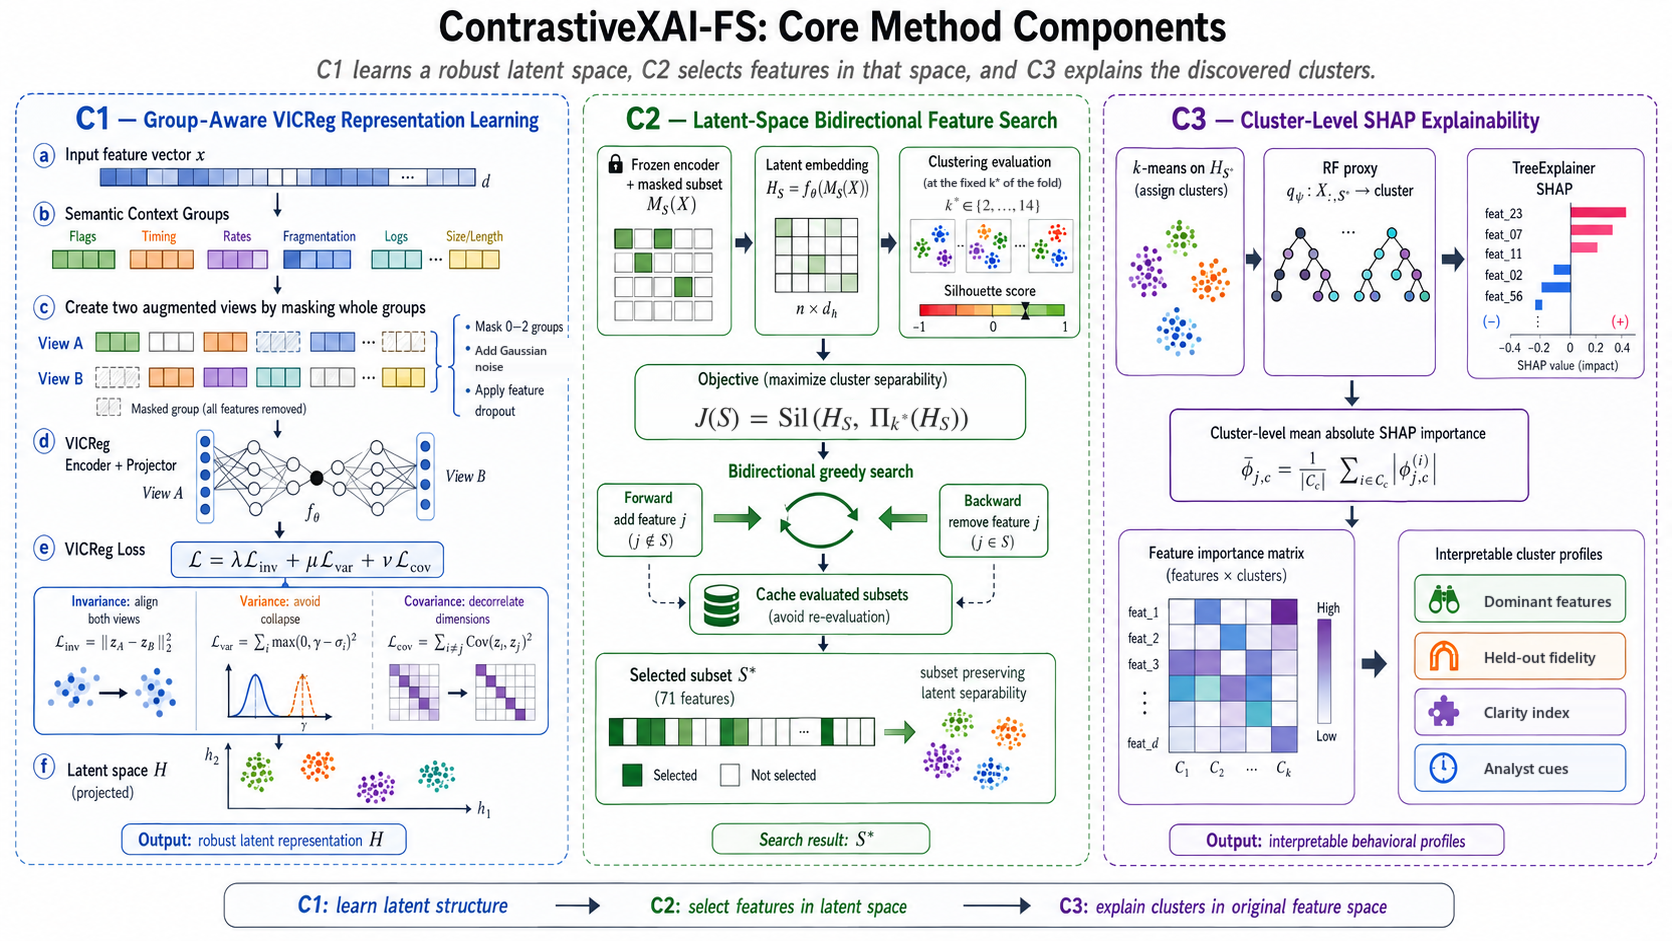
\includegraphics[width=0.95\textwidth]{figures/fig2_pipeline.png}
\caption{Overview of the proposed \method{} pipeline.}
\label{fig:pipeline}
\end{figure*}

\subsection{Group-Aware Semantic Augmentation}
\label{sec:augmentation}

In tabular IIoT traffic, perturbing isolated features can produce semantically inconsistent samples. For example, changing a TCP flag statistic without modifying related flag counts may create an unrealistic protocol state. To reduce this risk, \method{} masks complete semantic Context Groups, while individual feature dropout and Gaussian noise are retained as lower-amplitude complementary perturbations. Let $\mathcal{B} \subseteq \mathcal{G}$ be a set of Context Groups sampled for masking, and let $U(\mathcal{B}) = \bigcup_{G_r \in \mathcal{B}} G_r$ be the union of the feature indices contained in these groups. For each augmented view, the number of masked groups is sampled as
\begin{equation}
m \sim \mathrm{Uniform}\{0, 1, 2\},
\end{equation}
and $m$ groups are then selected uniformly from $\mathcal{G}$ without replacement. The two augmented views of the same sample independently sample their masked groups. Given a standardized input $x$, the augmented view $\tilde{x} = \mathcal{A}(x)$ is defined component-wise as
\begin{equation}
\tilde{x}_j =
\begin{cases}
0, & \text{if } j \in U(\mathcal{B}),\\
r_j\,(x_j + \eta_j), & \text{otherwise},
\end{cases}
\label{eq:augment}
\end{equation}
where $r_j \sim \mathrm{Bernoulli}(1 - p_{\mathrm{drop}})$ is an independent feature-dropout mask with $p_{\mathrm{drop}} = 0.10$ and $\eta_j \sim \mathcal{N}(0, 0.05^2)$ is Gaussian noise expressed in standardized feature units.

Group masking removes a complete semantic observation channel, such as timing, fragmentation, or flag behavior, rather than breaking the internal structure of a group; the Gaussian noise introduces small local variability in the surviving features; and feature dropout prevents the encoder from relying excessively on a small number of individual attributes. The augmentation does not assume that every perturbed vector corresponds to a complete executable network trace. Its purpose is to preserve the relationships among the unmasked measurement contexts while exposing the encoder to controlled uncertainty in the available observations.

\subsection{VICReg Encoder for IIoT Traffic Representation}

\method{} uses VICReg \cite{bardes2022vicreg} to learn a latent representation from unlabeled traffic windows. VICReg is a non-contrastive joint-embedding objective: it does not require negative pairs, and it explicitly penalizes representation collapse through a variance term. This property is useful in IIoT tabular traffic, where the semantic validity of augmentations is more difficult to guarantee than in image-based self-supervised learning.

Let $f_\theta : \mathbb{R}^{d} \rightarrow \mathbb{R}^{p}$ be the encoder and $g_\phi : \mathbb{R}^{p} \rightarrow \mathbb{R}^{r}$ be the projector, with $p = 128$ and $r = 512$. For each sample $x_i$, two augmented views $\tilde{x}_i = \mathcal{A}_1(x_i)$ and $\tilde{x}'_i = \mathcal{A}_2(x_i)$ are generated independently, producing $z_i = g_\phi(f_\theta(\tilde{x}_i))$ and $z'_i = g_\phi(f_\theta(\tilde{x}'_i))$. For a mini-batch of size $b$, let $Z = [z_1,\dots,z_b]^\top$ and $Z' = [z'_1,\dots,z'_b]^\top$. The VICReg loss is
\begin{equation}
\mathcal{L}_{\mathrm{VICReg}} = \lambda\,\mathcal{L}_{\mathrm{inv}}(Z,Z') + \mu\,\mathcal{L}_{\mathrm{var}}(Z,Z') + \nu\,\mathcal{L}_{\mathrm{cov}}(Z,Z').
\label{eq:vicreg}
\end{equation}
The invariance term encourages the two augmented views of the same sample to have similar projections:
\begin{equation}
\mathcal{L}_{\mathrm{inv}}(Z,Z') = \rev{\frac{1}{b\,r}}\sum_{i=1}^{b} \lVert z_i - z'_i \rVert_2^2 .
\end{equation}
The variance term prevents collapse by requiring each projection dimension to maintain sufficient variability within the mini-batch:
\begin{equation}
\mathcal{L}_{\mathrm{var}}(Z,Z') = \rev{\tfrac{1}{2}}\bigl[v(Z) + v(Z')\bigr],
\end{equation}
\begin{equation}
v(Z) = \frac{1}{r}\sum_{j=1}^{r} \max\!\Bigl(0,\; \gamma - \sqrt{\mathrm{Var}(Z_{:,j}) + \epsilon}\Bigr),
\end{equation}
where $\gamma = 1$ is the standard-deviation threshold and $\epsilon = 10^{-4}$ provides numerical stability. The covariance term decorrelates different projection dimensions:
\begin{equation}
\mathcal{L}_{\mathrm{cov}}(Z,Z') = \rev{\tfrac{1}{2}}\bigl[c(Z) + c(Z')\bigr], \qquad
c(Z) = \frac{1}{r}\sum_{i \neq j} [\mathrm{Cov}(Z)]_{ij}^2 ,
\end{equation}
where $\mathrm{Cov}(Z)$ is the empirical covariance matrix of the centered mini-batch projections. \rev{The normalization constants above are those of the implementation used in all experiments.} The weights are set to $\lambda = \mu = 25$ and $\nu = 1$, following the standard VICReg configuration.

The encoder is trained only on the training fold of each cross-validation split. \rev{For computational tractability on the CPU-only platform used in this study, each encoder is trained on a uniform random subsample of at most 20,480 training-fold rows, drawn without reference to labels.} After training, the projector $g_\phi$ is discarded, and only the frozen encoder output $h = f_\theta(x)$ is used for latent-space subset evaluation.

\subsection{Latent-Space Feature Subset Evaluation}
\label{sec:objective}

The method selects original traffic attributes rather than latent dimensions, but each subset of original features is evaluated through the frozen nonlinear representation. This design preserves the physical and operational meaning of the selected inputs while allowing the objective to reflect interactions among traffic measurements that may not be visible from independent feature scores or raw-space distances.

For a candidate subset $S$, unselected features are masked with the operator of Eq.~\eqref{eq:mask}, and the masked data are projected through the frozen encoder:
\begin{equation}
H_S = f_\theta(M_S(X)) \in \mathbb{R}^{n \times p}.
\end{equation}
For a number of clusters $k$, $k$-Means is fitted to $H_S$, producing a partition $\Pi_k(H_S)$ whose quality is measured with the Silhouette score \cite{rousseeuw1987silhouettes}. For each sample $i$, let $a(i)$ be the average distance from $i$ to all other samples in the same cluster, and let $b(i)$ be the smallest average distance from $i$ to the samples of any other cluster. Then
\begin{equation}
s(i) = \frac{b(i) - a(i)}{\max\{a(i), b(i)\}}, \qquad
\Sil(H_S, \Pi_k) = \frac{1}{n}\sum_{i=1}^{n} s(i).
\end{equation}

\rev{The number of clusters is selected once per training fold, using the complete feature set, over the candidate set $\mathcal{K} = \{2,\dots,14\}$:
\begin{equation}
k^{*} = \argmax_{k \in \mathcal{K}} \; \Sil\bigl(H_{[d]}, \Pi_k(H_{[d]})\bigr),
\label{eq:kstar}
\end{equation}
and it is then held fixed during the subset search, so that all candidate subsets are compared at the same partition granularity:
\begin{equation}
J(S) = \Sil\bigl(H_S, \Pi_{k^{*}}(H_S)\bigr).
\label{eq:objective}
\end{equation}
Eqs.~\eqref{eq:kstar} and \eqref{eq:objective} describe the procedure that is actually executed; they replace the per-subset maximization over $k$ stated in the previous version of this manuscript. To keep the search tractable, the objective is estimated on a fixed uniform subsample of the training fold: $k$-Means (five initializations) is fitted on 5,000 training rows, and the Silhouette score is computed on 2,000 of those rows. The same subsample and random seed are used for every candidate subset within a fold, so that $J(S)$ is a deterministic function of $S$.}

Silhouette is used because it provides an internal, label-free measure of cluster cohesion and separation. This criterion does not assume that maximizing Silhouette necessarily maximizes supervised classification performance; the relationship between this objective and downstream detection performance is assessed empirically. A candidate clustering is considered valid only when $k$-Means produces at least two nonempty clusters; invalid configurations are rejected, and subsets containing fewer than two features are not evaluated.

The ideal feature-selection problem, $S^{*} = \argmax_{S \subseteq [d]} J(S)$, cannot be solved exactly because it requires evaluating $2^{d}$ subsets. \method{} therefore uses a bidirectional greedy search that combines backward elimination with forward recovery.

\subsection{Bidirectional Silhouette-Based Search}
\label{sec:search}

The search is initialized with the complete feature set $S_0 = [d]$, which guarantees a valid initial representation. In the backward-removal pass, the algorithm evaluates $S \setminus \{j\}$ for every feature $j \in S$, provided that at least two features remain, and accepts the removal producing the largest strict improvement in $J(S)$. In the forward-recovery pass, it evaluates $S \cup \{j\}$ for every $j \notin S$ and restores the feature whose inclusion produces the largest strict improvement. The procedure alternates these passes until neither a removal nor a reintroduction improves the objective (Algorithm~\ref{alg:search}). All evaluated subsets are stored in a cache that is specific to the current training fold and frozen encoder.

\rev{Because a removal is accepted only when it strictly improves the objective and no cardinality penalty is applied, the search stops at a \emph{natural operating point} whose size is determined by the data. For comparisons at a prescribed cardinality, we use a budget-constrained variant: starting from the natural subset, the feature whose removal leaves the highest $J(S)$ is removed, even when $J$ decreases, until the requested budget is reached. To limit the number of evaluations, $\lfloor 0.1\,|S| \rfloor$ features are removed per pass while $|S| > 25$, and exactly one feature per pass thereafter. The same natural and budget-constrained procedures are applied in the standardized input space for the raw-space $k$-Means+Sil reference.}

\begin{algorithm}[t]
\caption{\method}
\label{alg:main}
\footnotesize
\begin{algorithmic}[1]
\Require Unlabeled training data $X_{\mathrm{tr}}$, Context Groups $\mathcal{G}$, candidate cluster set $\mathcal{K}$
\Ensure Selected subset $S^{*}$, cluster assignments $\hat{y}^{c}$, cluster profiles $\{P_c\}$
\State Fit imputation, infinite-value replacement, and standardization on $X_{\mathrm{tr}}$
\For{each training epoch}
  \For{each mini-batch $B \subset X_{\mathrm{tr}}$}
    \State Generate views $\tilde{B} = \mathcal{A}_1(B)$ and $\tilde{B}' = \mathcal{A}_2(B)$
    \State $Z \gets g_\phi(f_\theta(\tilde{B}))$, \; $Z' \gets g_\phi(f_\theta(\tilde{B}'))$
    \State Update $\theta, \phi$ by minimizing $\mathcal{L}_{\mathrm{VICReg}}(Z, Z')$
  \EndFor
\EndFor
\State Freeze $f_\theta$ and discard $g_\phi$
\State \rev{Select $k^{*}$ with Eq.~\eqref{eq:kstar}}
\State $S^{*} \gets \textsc{BidirectionalSearch}(X_{\mathrm{tr}}, f_\theta, k^{*})$
\State Fit $k$-Means with $k^{*}$ clusters on $H_{S^{*}} = f_\theta(M_{S^{*}}(X_{\mathrm{tr}}))$; obtain $\hat{y}^{c}$
\State \rev{Split the clustered rows into proxy-training and held-out parts}
\State Train Random Forest proxy $q_\psi : X_{:,S^{*}} \rightarrow \hat{y}^{c}$ \rev{on the proxy-training part}
\State \rev{Measure proxy fidelity and compute TreeExplainer SHAP on the held-out part}
\State Compute cluster profiles $\{P_c\}$ \rev{and clarity indices $\{CI_c\}$}
\State \Return $S^{*}$, $\hat{y}^{c}$, $\{P_c\}$
\end{algorithmic}
\end{algorithm}

\begin{algorithm}[t]
\caption{Bidirectional Latent Silhouette Search}
\label{alg:search}
\footnotesize
\begin{algorithmic}[1]
\Require Training data $X$, frozen encoder $f_\theta$, \rev{fixed $k^{*}$}, feature set $[d]$
\Ensure Selected feature subset $S^{*}$
\State $S \gets [d]$; cache $\mathcal{C} \gets \emptyset$; compute and cache $J(S)$
\State $improved \gets$ \textbf{true}
\While{$improved$}
  \State $improved \gets$ \textbf{false}
  \State $S_{\mathrm{best}} \gets S$; $J_{\mathrm{best}} \gets J(S)$ \Comment{Backward-removal pass}
  \For{each feature $j \in S$ with $|S| > 2$}
    \State $S' \gets S \setminus \{j\}$; compute $J(S')$ with Eq.~\eqref{eq:objective} if $S' \notin \mathcal{C}$
    \If{$J(S') > J_{\mathrm{best}}$} $S_{\mathrm{best}} \gets S'$; $J_{\mathrm{best}} \gets J(S')$ \EndIf
  \EndFor
  \If{$S_{\mathrm{best}} \neq S$} $S \gets S_{\mathrm{best}}$; $improved \gets$ \textbf{true} \EndIf
  \State $S_{\mathrm{best}} \gets S$; $J_{\mathrm{best}} \gets J(S)$ \Comment{Forward-recovery pass}
  \For{each feature $j \in [d] \setminus S$}
    \State $S' \gets S \cup \{j\}$; compute $J(S')$ with Eq.~\eqref{eq:objective} if $S' \notin \mathcal{C}$
    \If{$J(S') > J_{\mathrm{best}}$} $S_{\mathrm{best}} \gets S'$; $J_{\mathrm{best}} \gets J(S')$ \EndIf
  \EndFor
  \If{$S_{\mathrm{best}} \neq S$} $S \gets S_{\mathrm{best}}$; $improved \gets$ \textbf{true} \EndIf
\EndWhile
\State \Return $S$
\end{algorithmic}
\end{algorithm}

\subsection{Cluster-Level SHAP Explainability}
\label{sec:xai_method}

The final stage interprets the unsupervised cluster structure produced from the selected feature subset. After selecting $S^{*}$, the data are projected into the selected latent representation, $H_{S^{*}} = f_\theta(M_{S^{*}}(X))$, and a $k$-Means model with $k^{*}$ clusters produces the cluster assignments $\hat{y}^{c}_i \in \{1,\dots,k^{*}\}$.

Because the VICReg encoder is not directly interpretable in terms of original traffic features, we train a Random Forest proxy model $q_\psi$ to reproduce the cluster assignments using only the selected original features:
\begin{equation}
q_\psi : X_{:,S^{*}} \rightarrow \hat{y}^{c}.
\end{equation}
\rev{The proxy explanations describe the relationship between the selected original features and the latent cluster assignments. They do not explain the internal parameters or latent dimensions of the VICReg encoder, nor the sequence of decisions made by the subset search, and they do not establish a one-to-one correspondence between a latent cluster and an attack category. This scope applies to every explainability result reported in this paper and is not repeated in the following sections.}

\rev{To quantify how faithfully the proxy approximates the latent partition, the clustered rows are split, stratified by cluster, into a proxy-training part and a disjoint held-out part. The proxy is fitted on a cluster-balanced sample of the proxy-training part, and its fidelity is measured on the held-out part through accuracy, balanced accuracy, and per-cluster precision, recall, and F1 with respect to the latent cluster assignments. In the cross-validation experiments, fidelity is additionally measured on the outer test fold, whose rows are not seen by the scaler, the encoder, the subset search, the $k$-Means model, or the proxy.}

TreeExplainer SHAP \cite{lundberg2017unified} is then applied to the proxy model \rev{on held-out rows}. For sample $i$, feature $j$, and cluster $c$, the SHAP value $\phi^{(i)}_{j,c}$ estimates the contribution of feature $j$ to the proxy output for cluster $c$. SHAP values are aggregated at the cluster level using the mean absolute contribution,
\begin{equation}
\bar{\phi}_{j,c} = \frac{1}{|\mathcal{C}_c|}\sum_{i \in \mathcal{C}_c} \bigl|\phi^{(i)}_{j,c}\bigr| ,
\label{eq:clustershap}
\end{equation}
where $\mathcal{C}_c$ is the set of \rev{held-out} samples assigned to cluster $c$, and the behavioral profile of a cluster is the set of its top-$M$ features according to $\bar{\phi}_{j,c}$. Because the Context Groups contain different numbers of features, raw group-level SHAP sums are not used for cross-group ranking; the analysis relies on feature-level contributions.

\rev{Not every cluster yields a profile that an analyst can read. To avoid a subjective choice of which clusters to interpret, each cluster receives a \emph{clarity index}
\begin{equation}
CI_c = F_c \cdot T_c, \qquad
T_c = \frac{\sum_{j \in \mathrm{Top3}(c)} \bar{\phi}_{j,c}}{\sum_{j \in S^{*}} \bar{\phi}_{j,c}},
\label{eq:clarity}
\end{equation}
where $F_c$ is the held-out F1 of the proxy for cluster $c$ and $T_c$ is the share of the cluster's SHAP mass carried by its three most important features. $F_c$ measures whether the explanation is faithful to the latent cluster, and $T_c$ measures whether the profile is concentrated enough to be summarized by a few attributes. The index is reported for all clusters, and detailed interpretation is given in decreasing order of $CI_c$.}

\subsection{Computational Complexity and Scalability}
\label{sec:complexity}

The computational cost is divided into VICReg training, candidate-subset evaluation, and post-hoc proxy interpretation. Let $E$ denote the number of training epochs, \rev{$n_e$ the number of rows used for encoder training}, and $P$ the number of trainable parameters in the encoder and projector. For the fully connected architecture used here, representation learning costs approximately $O(E\,n_e\,P)$.

After training, the encoder is frozen. \rev{For one candidate subset, with $n_s$ rows used for clustering and $n_v \le n_s$ rows used for the Silhouette estimate, masking and encoding cost $O(n_s d + n_s P_f)$, where $P_f$ is the size of the frozen encoder; $k$-Means with $I$ iterations costs $O(I\,n_s\,p\,k^{*})$; and the Silhouette estimate costs $O(n_v^{2}\,p)$. One backward pass evaluates at most $|S|$ candidates and one forward-recovery pass at most $d - |S|$. If $T$ unique subsets are evaluated before convergence, the search costs $O\bigl(T\,(n_s d + n_s P_f + I\,n_s\,p\,k^{*} + n_v^{2}\,p)\bigr)$.} The cache ensures that each unique candidate is scored at most once within a fold. Increasing $d$ enlarges the number of neighboring subsets examined at each pass, whereas the subsampling makes the per-candidate cost independent of the training-fold size. \rev{The measured offline cost of these stages on the experimental platform is reported in Section~\ref{sec:cost}.}
